%%%%%%%%%%%%%%%%%%%%%%%%%%%%%%%%%%%%%%%%%
% Long Lined Cover Letter
% LaTeX Template
% Version 2.0 (September 17, 2021)
%
% This template originates from:
% https://www.LaTeXTemplates.com
%
% Authors: Fanchao Chen
% (chenfc@fudan.edu.cn)
%
% License:
% CC BY-NC-SA 4.0 (https://creativecommons.org/licenses/by-nc-sa/4.0/)
%
%%%%%%%%%%%%%%%%%%%%%%%%%%%%%%%%%%%%%%%%%

%----------------------------------------------------------------------------------------
%	PACKAGES AND OTHER DOCUMENT CONFIGURATIONS
%----------------------------------------------------------------------------------------

\documentclass[10pt]{article}

\usepackage{charter} % Use the Charter font
\usepackage{wrapfig}

\usepackage[
	a4paper,    % Paper size
	top=1in,    % Top margin
	bottom=1in, % Bottom margin
	left=.5in,   % Left margin
	right=.5in,  % Right margin
	%showframe  % Uncomment to show frames around the margins for debugging purposes
]{geometry}
\usepackage[hidelinks]{hyperref} 

\usepackage{enumitem}
\setitemize{noitemsep,topsep=0pt,parsep=0pt,partopsep=0pt}

\setlength{\parindent}{0pt}     % Paragraph indentation 
\setlength{\parskip}{1em}       % Vertical space between paragraphs

\usepackage{graphicx}       % Required for including images

\usepackage{fancyhdr}       % Required for customizing headers and footers

\fancypagestyle{firstpage}{%
	\fancyhf{} % Clear default headers/footers
	\renewcommand{\headrulewidth}{0pt} % No header rule
	\renewcommand{\footrulewidth}{0pt} % Footer rule thickness
}

\fancypagestyle{subsequentpages}{%
	\fancyhf{} % Clear default headers/footers
	\renewcommand{\headrulewidth}{1pt} % Header rule thickness
	\renewcommand{\footrulewidth}{1pt} % Footer rule thickness
}

\AtBeginDocument{\thispagestyle{firstpage}} % Use the first page headers/footers style on the first page
\pagestyle{subsequentpages} % Use the subsequent pages headers/footers style on subsequent pages

%----------------------------------------------------------------------------------------
\usepackage[framemethod=tikz]{mdframed}
\begin{document}
%\thispagestyle{none}
\pagestyle{plain}

%----------------------------------------------------------------------------------------
%	FIRST PAGE HEADER
%----------------------------------------------------------------------------------------

\begin{minipage}{4in}

\includegraphics[width=4in]{waterloo.png}
\end{minipage}\begin{minipage}{1in}
~
\end{minipage}\begin{minipage}{3in}
{\bf Prof. Jo Atlee}\\ 
Tel.   +1 (519) 888-4567\\
Email: jmatlee@uwaterloo.ca\\
URL: https://cs.uwaterloo.ca/~jmatlee/\\~\\
 October 30, 2024
\end{minipage}
\vspace{0.5in}

%----------------------------------------------------------------------------------------
%	ADDRESSEE AND GREETING
%----------------------------------------------------------------------------------------
To whom it may  concern

\bigskip % Vertical whitespace

%----------------------------------------------------------------------------------------
%	LETTER CONTENT
%----------------------------------------------------------------------------------------

I write to nominate Prof. Tim Menzies(IEEE member number 41349237,
timm@ieee.org, +1-304-376-2859) of North Carolina State University,
for the IEEE TCSE Lifetime Achievement  Award. 
% \begin{mdframed}[hidealllines=true,backgroundcolor=blue!10]
% \begin{center}
% {\bf Proposed Citation:}
% {\em For contributions to the foundation and application of AI to Software Engineering}
% \end{center}
% \end{mdframed}
% This package
% contains my nomination text and endorsement text from:
%
% \begin{itemize}
% \item  Prof Ahmed E. Hassan, Queen's University, ACM Fellow and IEEE Fellow
% \item Prof. Massimiliano (Max) Di Penta
% University of Sannio, Italy
% \item  Prof, Prem Devanbu, UC Davis, USA, ACM Fellow  (please note that Prof. Devanbu won this award in 2021). 
% \end{itemize}
%
%
My proposed citation for that award would be:

\begin{mdframed}[hidealllines=true,backgroundcolor=blue!10]
\begin{center}
{\em For outstanding fundamental reseaerch contributions in SE analytics.}
\end{center}
\end{mdframed}
 
In support of that award, this package contains:

\begin{enumerate}
\item
A paragraph explaining why the nominee deserves the recommended award.
\item
Letter from nominee, accepting the nomination.
\item
My supporting letter.
\item
Supporting letters from two referees.
\item
The vitae of the applicant.
\end{enumerate}

  % Vertical whitespace

Sincerely yours,


\includegraphics[width=4cm]{msig.png} % Logo


%\includegraphics[height = 1cm]{YourSignature.pdf}
%上面的YourSignature,请上传你自己的签名,导入到这里, 没有的话也可忽略。

Jo Atlee\\
Professor, University of Waterloo
%Department of Computer Science\\
%City University of Hong Kong

\newpage
\section{A paragraph explaining why the nominee deserves the recommended award.}


Decades before the IEEE (or the mining software repositories
community) advocated for open science standards, Menzies was an
early adopter of open science, always publishing his papers’ scripts
and data.
By his example, Menzies 
\textcolor{red}{{\bf raised the bar in software analytics to a new level}}. 
Decades before the IEEE (or the mining software repositories community) were advocating for open science standards, 
Menzies was an early adopter of open science, always publishing his papers’ scripts and data. 
His methods were copied by hundreds of other researchers (e.g. his 2006 work\footnote{
%[Me06] 
Citations = 1891. 	
Menzies, T., et al. (2006) “Data mining static code attributes to learn defect predictors”. IEEE Trans SE 33(1), 2-13 } is a 20 top-most cited paper in SE in cites/year). 
By 2017, a fifth of the top Google Scholar Metrics papers (in IEEE Transactions on SE) used artifacts popularized and published by Menzies.
Using this data, Menzies made many novel and important contributions.
For SE applications, he showed that
\textcolor{red}{{\bf applying standard AI approaches “out of the box” is not advisable for SE. Rather, AI should be customized for SE data and 
applications}}. For example, 
Menzies’ methods exploit “repetitions” in SE artifacts. 
Maintainable software contains repeated copies of structures familiar to many developers. 
Within similar regions, Menzies’ methods sample sparingly before quickly moving on elsewhere. This approach finds better models, orders of 
magnitude faster than the prior state of the art \footnote{
%[Me08] 
Citations = 426. 	Menzies, T. et al.. (2008) "Automated severity assessment of software defect reports." ICSME’08 } \footnote{
%[Me09] 
Citations = 856.
T Menzies, et al.(2009)  Relative value of cross-company and within-company data for defect prediction.    Empirical Software Engineering 14, 540-578
} \footnote{
%[Me10] 
citations = 589. 	  Menzies, T., et al. (2010)  "Defect prediction from static code features." Automated Software Engineering 17: 375-407. 
} \footnote{
%[Me20] 
Citations = 151.  T. Menzies   et al. (2020) "Finding Faster Configurations Using FLASH," in IEEE TSE, 46(7), pp. 794-811, 1  }
. For example:
In 2012, when applied at NASA, Menzies’ repetitions-aware technology found critical errors in the Space Shuttle’s pad abort system.
% In 2019, the ICSME conference gave his 2008 paper a “most influential” award \footnote{
% % %[Me08] 
% Citations = 426. 	Menzies, T. et al.. (2008) "Automated severity assessment of software defect reports." ICSME’08}.
As part of this work on SE and AI, Menzies found that many SE data
mining papers are not reproducible since their code and data was
unavailable. To address that, Menzies developed PROMISE-- a public
repository of software data as well as the PROMISE conference series
That data was used for decades, in thousands of papers, by other
researchers (see the 1,273 citations to  PROMISE repository\footnote{
\url{https://scholar.google.com/citations?user=7htTUTgmLtUC&hl=en&authuser=2}
} , as of Oct’24).
In recognition of his work, in 2017 the SE mining software repositories community awarded him the Foundational 
Contribution Award for “fundamental contributions in mining software repositories which helped others advance the state of the art.” 









\newpage
\section{A letter from nominees, accepting the nomination.}

\vspace{0.5in}
~\hrule~

\begin{minipage}{2.25in}

\includegraphics[width=2in]{logo.png}
\end{minipage}\begin{minipage}{3.75in}
{\bf Department of Computer Science} ~\\~\\~\\~\\~\\
\end{minipage}\begin{minipage}{2in}
{\bf Prof. Tim Menzies}\\ 
 timm@ieee.org\\ +1-304-376-2859	\\
 ~\\
 ~\\
 October 30, 2024
\end{minipage}
\vspace{1in}

To the IEEE TCSE awards committee.

I write to accept this nomination for the TCSE lifetime achivement award. 

For the committee's information, I assert my reseaerch
career began in 1988 \footnote{Tim Menzies, M. Dean, J. L. Black, J. F. Fleming:
Combining Heuristics and Simulation Models: An Expert System for the Optimal Management of Pigs. 
AJCAI 1988: 48-61} 
(and I switched to SE in 1993 \footnote{Tim Menzies, Julian M. Edwards, Kekwee Ng:
The Mysterious Case of the Missing Reusable Class Libraries. TOOLS (12/9) 1993: 421-427.}
\footnote{
Tim Menzies, Steve M. Easterbrook, Bashar Nuseibeh, Sam Waugh:
An Empirical Investigation of Multiple Viewpoint Reasoning in Requirements Engineering. IEEE RE 1999.}).
Hence, I my career is longer than the 25 years required for this award.

Yours sincerely,



\includegraphics[width=2.5in]{sig.png}


Tim Menzies



\newpage
\section{Support letter from nominator.}

\vspace{0.2in}
~\hrule~

\begin{minipage}{4in}

\includegraphics[width=4in]{waterloo.png}
\end{minipage}\begin{minipage}{1in}
~
\end{minipage}\begin{minipage}{3in}
{\bf Prof. Jo Atlee}\\ 
Tel.   +1 (519) 888-4567\\
Email: jmatlee@uwaterloo.ca\\
URL: https://cs.uwaterloo.ca/~jmatlee/\\~\\
 October 30, 2024
\end{minipage}
\vspace{0.5in}

To the IEEE TCSE awards committee.

I write to nominate Prof. Tim Menzies(IEEE member number 41349237) for the IEEE TCSE Lifetime Achievement  Award. 
My proposed citation for that award is:

\begin{mdframed}[hidealllines=true,backgroundcolor=blue!10]
\begin{center}
{\em For outstanding fundamental reseaerch contributions in SE analytics.}
\end{center}
\end{mdframed}

In a research career dating back 1987 \footnote{A micro-computer, rule-based prolog 
expert-system for process control in a petrochemical plant
T Menzies, B Markey
Proceedings of the Third Australian Conference on Expert Systems, May 13-15, 1987.},
Menzies was (and continues to be) a pioneer and early adopter of using innovative AI methods for SE. In recognition of his work, in 2017 the SE mining software repositories community awarded him the Foundational Contribution Award for “fundamental contributions in mining software repositories which helped others advance the state of the art.” 
Menzies was one of the first SE researchers to report that data miners can find very strong signals within SE project data:
 \begin{itemize}
 \item
Menzies was one of the first to find defect predictors demonstrably better than humans (his 2006 IEEE TSE paper on that topic s a 20 top-most cited paper in SE in cites/year and 1891 total cites). 
\item
Menzies was one of the first to apply Pareto reasoning for trading-off software requirements 
\footnote{
% %[Me02] 
 Citations = 119. 	Menzies T. et.al . (2002) "Converging on optimal attainment of requirements." RE’02 }. 
\begin{itemize} 
\item 
Using novel mulit-objectve optimizers based on rule-based data mining algorithms, Menzies found he could out-perform the state-of-the-art to find better optimizations, in orders of magnitude less time  \footnote{
% %[Me20] 
 Citations = 151. T. Menzies and V. Nair et al. (2020)  "Finding Faster Configurations Using FLASH," in IEEE TSE, 46(7), pp. 794-811, 1 },


\item When applied at NASA in 2012, these methods found critical errors in the Space Shuttle pad abort system.
\end{itemize}
\item
In 2019, the ICSME conference gave Menzies’ 2008 paper a “most influential” award. That text mining work defined a cheap “occasional second opinion” policy for finding more bugs in code comments, quicker. 
\item
Menzies was the first to demonstrate large scale transfer learning of models between SE projects in different continents (see his 2009 EMSE paper).  
%\footnote{
% % %[Me09] 
% Citations = 778.  T Menzies, et al.  (2009)  Relative value of cross-company and within-company data for defect prediction.  Empirical Software Engineering 14, 540-578
% }
\item
Menzies' research has been applied commercially around the world. 
\begin{itemize}
    \item  
Turkish researchers found that when commercial teams restricted code inspections to 25 percent of the files identified using Menzies’ algorithms, they found 88\% of the existing code defects in software. 
\item Those defect prediction methods have been commercialized and deployed at 
Chevron, Northrop Grumman, LogLogic, Inc., and Compagnie Financi\'ere Alcatel.
\end{itemize}
\end{itemize}

Decades before the ACM (or the mining software repositories community) advocated for open science standards, Menzies was an early adopter of open science, always publishing his papers’ scripts and data. Accordingly:
\begin{itemize}
    \item  
 His methods have been widely cited. For example, his IEEE TSE 2006 paper currently has 1891 citations.
\item His methods have been widely copied. By 2017, a fifth of the top Google Scholar Metrics papers (in IEEE Transactions on SE) used artifacts popularized and published by Menzies 
\item As part of this work on SE + AI, Menzies found that many SE data mining papers are not reproducible since their code and data was unavailable. To address that, Menzies developed PROMISE-- a public repository of software data as well as the PROMISE conference series That data was used for decades, in thousands of papers, by other researchers (see the 1,273 citations to  PROMISE repository\footnote{
% %[Me12]	
\url{https://scholar.google.com/citations?user=7htTUTgmLtUC&hl=en&authuser=2}
} , as of July’23).
\end{itemize}


Menzies’ research teaches us that SE is subtly different to many of the problems students in the AI community, Hence, as shown in many of his papers, it is best to customize AI before applying it to SE. For example:
\begin{itemize}
    \item  
Optimization methods for numerical systems have been used widely. But applying these methods is often ineffective in complex software systems where each "if" statement divides the software into regions with different properties. Fortunately, many of those regions contain repeated structures. Menzies’ nonparametric optimizers exploit that repetition (by learning regions of similarity and knowing when to jump to other regions)  (see his RE'02 paper).
\item 
In this way, Menzies’ optimizers can quickly learn how to make code run quicker, make web servers handle more traffic, and compile programs faster  (see his 2020 IEEE TSE article) (even for systems with millions of configuration options). 
\end{itemize}



 
To say the least, his work is highly cited.
Garousi and  Fernandes\footnote{\url{https://www.sciencedirect.com/science/article/pii/S0950584915001871}}  list Menzies' IEEE 2006 Transactions on Software Engineering paper as one of the top 100 most-cited SE papers of all time:
\begin{itemize}
\item
From  2009 to 2019, this paper had the most cites/year of any IEEE Transactions on Software Engineering paper (and for SE overall, it is a top-20 most cites/year paper).
\item At the time of this writing (2023), measured in terms of citations/year,   that 2006 paper   ranks number two (in Google Scholar metrics for Software Systems for the TSE journal). 
\end{itemize}  


Menzies has been acknowledged by our community as follows:

\begin{itemize}
\item an IEEE Fellow award (2018); 
\item an ASE Fellow award (2023); 
\item a Foundational Contribution Award from the Mining Software repositories community (2017); 
\item an award from NASA headquarters from NASA’s Chief of Mission Assurance (2005) 
\item distinguished paper awards at the top conferences in his field (FSE’21, ICSE’19, ICMSE’19); 
\item awards for his work on conference and journal reviewing (2011-2018)
\item Appointment, editor in chief, Automated Software Engineering journal.
\end{itemize}
Details follow:
\begin{itemize} 
\item 2023: appointed Automated Software Engineering Fellow
\item 2021: Appointment, editor in chief, Automated Software Engineering journal.
\item
2021: distinguished (best) paper award, FSE;
\item 2019: distinguished (best) paper award, International Conference on Software Engineering.
\item 2019: a ``most influential''  award for  "Automated severity assessment of software defect reports”, ICSME'09
\item 2018: appointed IEEE Fellow
\item 2017: MSR (Mining Software Repositories) Foundational Contribution Award in "Recognition of fundamental contributions in the field of data mining software repositories which helped others advance the state of the art.”
\item 2011-2018: distinguished reviewer, ACM TOSEM (only person to be awarded this for each year 2011 to 2018). 
\item 2005: As science chair at a NASA facility, Menzies received a commendation award from NASA’s Chief  of Safety and Mission Assurance (and former Space Shuttle Pilot) 
Byran O'Connor saying: 
\end{itemize}
\begin{mdframed}[hidealllines=true,backgroundcolor=blue!10]
\begin{center}
\begin{quote}
{\em 
    "...A great researcher in his own right, ...Tim has raised the bar on quality and level of work [expected] from our researchers."} 
\end{quote}
\end{center}
\end{mdframed}

Sincerely yours,


\includegraphics[width=4cm]{msig.png} % Logo


%\includegraphics[height = 1cm]{YourSignature.pdf}
%上面的YourSignature,请上传你自己的签名,导入到这里, 没有的话也可忽略。

Jo Atlee\\
Professor, University of Waterloo
%Department of Computer Science\\
%City University of Hong Kong


\newpage
\section{a. Referee letter \#1.}

\begin{wrapfigure}{r}{2.8in}
\vspace{-.6in}

\includegraphics[width=2.8in]{img/aheader.png}
\vspace{-.7in}
\end{wrapfigure}

{ 
~\\~\\~\\~\\~\\
October 21, 2024

 

{\bf RE: Endorsement of Dr. Tim Menzies’ Nomination}

 

Dear Member of the Adjudication Committee,
 
 





I strongly support the nomination of Dr. Menzies who has been
instrumental in shaping the research agenda of Software Engineering
(SE). His influence extends beyond his ground-breaking research,
which continues to have a profound impact on both industry and
academia, and through his unwavering spearheading of vital initiatives
within our community.



In today's era, marked by the ubiquity of platforms like GitHub,
the widespread use of data analytics, it's easy to forget that just
two decades ago, obtaining project data and applying data science
approaches were rare and the domain of highly specialized experts.
However, in 2005, Dr. Menzies embarked on a mission to gather data
for the PROMISE repository. He reached out to potential data providers
and meticulously scanned the tables of contents of conference
proceedings. This collaborative effort, initially undertaken by
himself then his students, led to the establishment of the PROMISE
repository. Today, this repository is home to a vast collection of
shareable data covering a range of domains, including defect
prediction, effort estimation, and requirements models. The PROMISE
repository stands as a monumental achievement that has played a
pivotal role in shaping the landscape of defect prediction and
software effort estimation, providing invaluable resources and
accelerating the progress of knowledge.



In contrast to those who treat machine learning as a black-box tool,
Dr. Menzies and his team are dedicated to a hands-on approach,
deeply understanding the domain and problems before carefully
selecting from a range of algorithms, rather than resorting to
off-the-shelf solutions.  For example, in his 2017 FSE paper, "Easy
over hard: a case study on deep learning," Dr. Menzies raised
awareness about the risks of using machine learning as a black-box
tool and advocated the exploration of simpler, faster techniques
before resorting to deep learning methods in SE tasks.



Dr. Menzies is distinguished as one of the 15 most active IEEE
fellows in the SE field. He has co-authored many highly cited papers.
Recent assessments by Elsevier position him as a leading figure in
SE research over the past decade and the 11th most active researcher
in the field based on high-impact journal publications. Dr. Menzies'
profound impact on the mining software repositories field was honored
with the MSR Foundational Contribution Award. One of his original
papers on the PROMISE repository is now among the 100 most cited
papers in the history of SE.



I wholeheartedly endorse him for this award. His research and
commitment to open, collaborative, and constructive research
evaluation is unparalleled, has had an enormously positive impact
on SE.



Best regards,

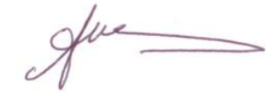
\includegraphics[width=2in]{img/asig.png}\newline
Ahmed E. Hassan, PhD, {\bf ahmed@cs.queensu.ca}\newline
Mustafa Prize Laureate, Fellow of IEEE, ACM, AAIA and NSERC Stacie\newline
ACM SIGSOFT Influential Educator, IEEE TCSE Distinguished Educator\newline
Member of the New College of the Royal Society of Canada\newline
Canada Research Chair in Software Analytics\newline
School of Computing, Queen's University, Kingston Ontario, Canada 

\begin{center}
  
\includegraphics[width=\linewidth]{img/afooter.png}  
\end{center}
}

\newpage
\section{b. Referee letter \#2.}


\hspace{-1cm}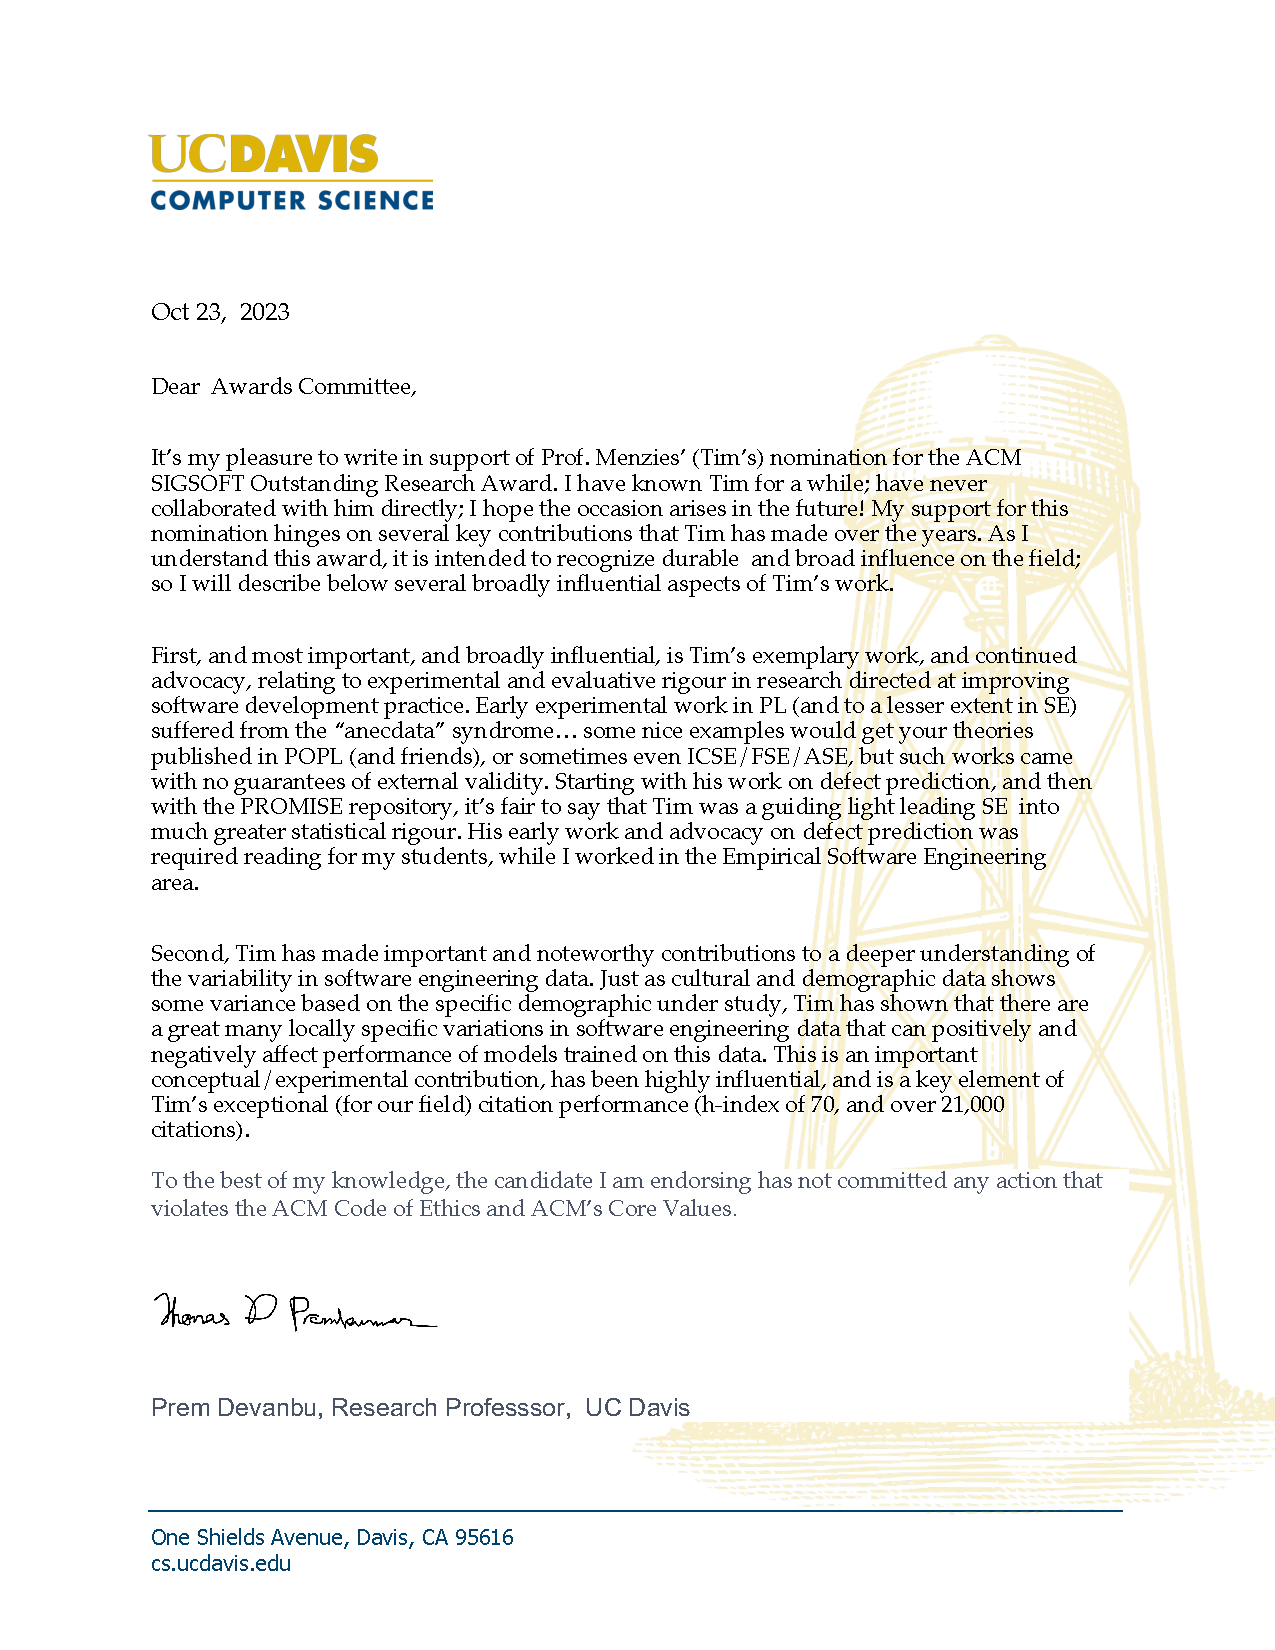
\includegraphics[width=8in]{menzies-sigsoft.pdf}

\newpage
\section{Vitae of nominee.}



\end{document}
